\input{preambule_damien2.tex}     

%%%%%%%%%%%%%%%%%%%%%%%%%%%%%%%%%%%%%%%%%%%
%****************TABLEAUX*******************************%
%%%%%%%%%%%%%%%%%%%%%%%%%%%%%%%%%%%%%%%%%%%

%%%%%%%%%%%%%%%% TABLEAU SIGNE ET VARIATION %%%%%%%%%%%%%%
%\begin{center}
%%\vspace{0.3cm}
%\begin{tikzpicture}
%\tkzTabInit[espcl=2]{$x$ /.8 , $d(x)$ /1.5}{$0$ , $4$,$16$,$24$}
%\tkzTabLine[]{,+,z,-,}
%\tkzTabVar[]{+/ $8$,-/$6$,+/$19$,-/$8$}
%%\tkzTabVal[draw]{1}{2}{0.5}{0}{0}
%\end{tikzpicture}
%\end{center}

%%%%%%%%%%%%%%% TABLEAU %%%%%%%%%%%%%%%%%%%%%%%%%%%%%%
%\renewcommand{\arraystretch}{hauteur}
%\begin{center}
%\begin{tabularx}{0.94\linewidth}{|c|*{7}{>{\centering \arraybackslash}X|}}
%\hline 
%
%\hline 
%\end{tabularx} 
%\end{center}

%%%%%%%%%%%%%%%%%%%%%%%%%%%%%%%%%%%%%%%%%%%
%****************** GRAPHIQUE FCT**********************%
%%%%%%%%%%%%%%%%%%%%%%%%%%%%%%%%%%%%%%%%%%%

%\psset{xunit=0.75cm,yunit=0.75cm,algebraic=true,dimen=middle,dotstyle=o,dotsize=5pt 0,linewidth=1.4pt,arrowsize=2pt 2,arrowinset=0.25}
%\def\xmin{-9} \def\xmax{9} \def\ymin{-10.5} \def\ymax{6.5} \def\dx{0.5} \def\dy{0.5}
%\begin{center}
%		\begin{pspicture*}(\xmin,\ymin)(\xmax,\ymax)
%		\multips(0,\ymin)(0,\dy){35}{\psline[linestyle=dashed,linecap=1,dash=1.5pt 1.5pt,linewidth=0.4pt,linecolor=lightgray]{c-c}(\xmin,0)(\xmax,0)}
%		\multips(\xmin,0)(\dx,0){38}{\psline[linestyle=dashed,linecap=1,dash=1.5pt 1.5pt,linewidth=0.4pt,linecolor=lightgray]{c-c}(0,\ymin)(0,\ymax)}
%		\psaxes[labels=all,labelFontSize=\scriptstyle,labelsep=2pt,xAxis=true,yAxis=true,Dx=1,Dy=1,ticksize=-2pt 0,subticks=2,showorigin=False]{->}(0,0)(\xmin,\ymin)(\xmax,\ymax)[{$x$,0][$y$,90]
%\psclip{%
%\psframe[linestyle=none](\xmin,\ymin)(\xmax,\ymax)}
%		\uput[dl](0,0){\scriptsize $0$}
%		\psplot[linewidth=1.4pt,plotpoints=200, linecolor=blue]{\xmin}{\xmax}{2.79^x}
%}\endpsclip
%		\end{pspicture*}
%\end{center}

%%%%%%%%%%%%%%%%%%%%%%%%%%%%%%%%%%%%%%%%%%%
% *******************MINTED *****************************%
%%%%%%%%%%%%%%%%%%%%%%%%%%%%%%%%%%%%%%%%%%%
\usepackage{minted}
%
\renewcommand{\theFancyVerbLine}{\textcolor{gray}{\tiny \oldstylenums{\arabic{FancyVerbLine}}}}
%
\definecolor{bg}{rgb}{0.95,0.95,0.95}
%
\newminted[python]{python}{fontfamily=tt,linenos=true,autogobble,mathescape=true,python3,fontsize=\small, tabsize=4, samepage=true, rulecolor=gray, numbersep=2pt, bgcolor=bg}
%
\newmintinline{python}{fontfamily=tt,linenos=true,autogobble,mathescape=true,python3}
%
%\newmintedfile[pythonexternal]{python}{fontfamily=tt,linenos=true,autogobble,mathescape=true,python3}
%
%\newminted[html]{html}{fontfamily=courier, fontsize=\footnotesize, rulecolor=gray, framerule=1.5pt, mathescape=true, texcomments=true, autogobble, tabsize=4, numbersep=8pt}
%
%\newmintinline{html}{fontfamily=courier, fontsize=\small}
%
%\newminted[css]{css}{fontfamily=courier, fontsize=\footnotesize, rulecolor=gray, framerule=1.5pt, mathescape=true, texcomments=true, autogobble, tabsize=4, numbersep=8pt}
%
%\newmintinline{css}{fontfamily=courier, fontsize=\small}
%
%\newminted[algo]{bbcode}{fontfamily=courier, fontsize=\footnotesize, rulecolor=gray, framerule=1.5pt, mathescape=true, texcomments=true, autogobble, linenos=true, tabsize=4, numbersep=8pt}

%%%%%%%%%%%%%%%%%%%%%%%%%%%%%%%%%%%%%%%%%%%
% *******************EnT�tes et Pieds de page *****************************%
%%%%%%%%%%%%%%%%%%%%%%%%%%%%%%%%%%%%%%%%%%%
\pagestyle{fancy}
\setlength{\headheight}{40pt} % Haut de page
\renewcommand{\headrulewidth}{0.0pt}
\setlength{\textheight}{26cm}
\lhead{}
%\chead{\thepage/\pageref{LastPage}}
\rhead{}
\renewcommand{\footrulewidth}{1pt}
\lfoot{2GT --- SNT}
\cfoot{}
%\rfoot{\thepage/\pageref{LastPage}}


%%%%%%%%%%%%%%%%%%%%%%%%%%%%%%%%%%%%%%%%%%%%%%

\begin{document}

\section*{Les R�seaux sociaux -- Entra�nement --- CORRECTION}

\begin{exo}[Questions de cours]
Voir le cours. Posez moi des questions si n�cessaire.
\end{exo}

\begin{exo}
\begin{em}
Une petite compagnie a�rienne propose des vols entre les a�roports de Paris, Lille, Bordeaux, Toulouse. De Paris, il est possible de rejoindre n'importe quelle autre ville (et inversement). De plus, un vol relie Bordeaux � Toulouse (dans les deux sens).

Repr�senter la situation par un graphe, o�, les sommets du graphe sont les villes desservies par la compagnie a�rienne, et les ar�tes sont les vols propos�s par la compagnie entre les diff�rente ville.
\end{em}

\begin{multicols}{2}
La solution se trouve ci-contre, o� les villes ont �t� repr�sent�es par leur initiale.

\begin{center}
  \begin{tikzpicture}[scale=2,very thick]
    \tikzset{sommet/.style={draw, circle, inner sep=2pt}}
    \tikzset{arete/.style={black}}
    \node[sommet] (P) at (1, 0) {P};
    \node[sommet] (T) at (0, 0) {T};
    \node[sommet] (B) at (0, 1) {B};
    \node[sommet] (L) at (1, 1) {L};
    \draw[arete] (B) -- (T);
    \draw[arete] (P) -- (T);
    \draw[arete] (P) -- (B);
    \draw[arete] (P) -- (L);
  \end{tikzpicture}
\end{center}
\end{multicols}
\end{exo}

\begin{exo}
  \begin{multicols}{2}
\begin{em}
Lors d'une soir�e, neuf invit�s s'amusent � tracer le graphe ci-contre, o� :
\begin{itemize}
  \item les sommets repr�sentent les neuf invit�s (repr�sent�s ici par des lettres) ;
  \item une ar�te entre deux invit�s signifie qu'ils se connaissaient avant la soir�e.
\end{itemize}
\end{em}

\columnbreak

\begin{center}
  \begin{tikzpicture}[scale=1.5,very thick]
    \tikzset{sommet/.style={draw, circle, inner sep=2pt}}
    \tikzset{arete/.style={black}}
    \node[sommet] (A) at (0, 2) {A};
    \node[sommet] (B) at (1, 2) {B};
    \node[sommet] (C) at (2, 2) {C};
    \node[sommet] (D) at (0, 1) {D};
    \node[sommet] (E) at (1, 1) {E};
    \node[sommet] (F) at (2, 1) {F};
    \node[sommet] (G) at (0, 0) {G};
    \node[sommet] (H) at (1, 0) {H};
    \node[sommet] (I) at (2, 0) {I};
    \draw[arete] (A) -- (B);
    \draw[arete] (B) -- (C);
    \draw[arete] (B) -- (E);
    \draw[arete] (C) -- (F);
    \draw[arete] (D) -- (E);
    \draw[arete] (G) -- (E);
    \draw[arete] (F) -- (I);
    \draw[arete] (H) -- (I);
  \end{tikzpicture}
\end{center}
\end{multicols}

\begin{em}
En justifiant, donner : le centre, le rayon, le diam�tre du graphe.
\end{em}

Commen�ons par calculer l'�cartement de chacun des sommets.
\begin{center}\begin{tabular}{r*{9}{c}}
    \toprule
    Sommet & A & B & C & D & E & F & G & H & I \\
    \midrule
    �cartement & 5 & 4 & 3 & 6 & 5 & 4 & 6 & 6 & 5 \\
    \bottomrule
\end{tabular}\end{center}

\begin{enumerate}
  \item Le diam�tre est le plus grand �cartement, soit \textbf{6}.
  \item Le centre est le sommet avec le plus petit �cartement, soit \textbf{C}.
  \item Le rayon est l'�cartement du centre, soit \textbf{3}.
\end{enumerate}
\end{exo}

\begin{exo}
  \begin{em}
Vous devez avoir suffisamment compris le document sur les bulles de filtres pour �tre capable de r�pondre � des questions du m�me genre.
\end{em}

Posez moi des questions si n�cessaire
\end{exo}

\end{document}